%! TEX root = course_report.tex

\section{Платформа Android}
\label{sec:android_platform}

ОС Android появилась более 15 лет назад.
Вскоре после этого права на ОС купила корпорация Google, увидев в ней огромный потенциал.
В результате на сегодняшний день Android -- самая популярная ОС для мобильных устройств с рыночной долей в 71\%, по данным StatCounter \cite{statcounter_mobile_os}.
StatCounter~-- сервис веб-аналитики, установленный на более чем 2 миллионах сайтов по всему миру.
Отчёты StatCounter основываются на данных веб-аналитики \cite{statcounter_methodology}.

Говоря об Android, обычно подразумевают платформу Android -- более широкое понятие, включающее в себя, помимо слоя абстракции оборудования (англ. \textit{Hardware Abstraction Layer}) и ядра, различные высокоуровневые средства для создания пользовательских приложений на языках Java и Kotlin.

\subsection{Структура и архитектура платформы}
\label{sub:android_platform:struct_and_arch}

Платформа Android состоит из нескольких слоёв абстракции, разделённых между собой для упрощения разработки каждого из них.
Далее будет рассмотрен каждый из этих слоёв.

\subsubsection{}
\label{subsub:android_platform:struct_and_arch:linux}
\textit{Ядро Linux} лежит в основе платформы Android.
Одна из причин использования ядра Linux -- широкие возможности Linux, нацеленные на повышение безопасности \cite{android_kernel_security}:
\begin{itemize}
	\item безопасное межпроцессное взаимодействие;
	\item изоляция приложений друг от друга;
	\item система прав доступа к файлам и папкам;
	\item защита загрузчика от несанкционированного изменения;
	\item современные криптографические алгоритмы.
\end{itemize}
Вместе со сборкой ядра Linux производители мобильных устройств поставляют драйверы оборудования (обычно в виде модулей с закрытым исходным кодом).

\subsubsection{}
\label{subsub:android_platform:struct_and_arch:hal}
\textit{Слой абстракции оборудования (HAL)} работает поверх ядра.
Он содержит библиотеки функций для более удобного доступа к оборудованию различных производителей из вышестоящих уровней абстракции.
HAL состоит из нескольких модулей, каждый из которых реализует интерфейс для определённого типа оборудования: камера, Bluetooth-модуль, микрофон, звуковой динамик и т. д. 

\subsubsection{}
\label{subsub:android_platform:struct_and_arch:art}
\textit{Android Runtime (ART)} -- среда выполнения Java и Kotlin приложений.
Она осуществляет компиляцию байт-кода ART в машинный код процессора, установленного в пользовательском устройстве.
ART пришла на cмену Dalvik в версии Android 5.0.
Одним из преимуществ ART по сравнению с Dalvik является компиляция приложений во время установки в машинный код устройства (англ. \textit{ahead-of-time}).
Это позволяет сократить время запуска приложения.
При этом установка приложений может занимать больше времени, чем при компиляции во время выполнения (англ. \textit{just-in-time}).

На одном уровне с \textit{ART} находятся \textit{системные C и C++ библиотеки}, предоставляющие высокоуровневый интерфейс для распространённых задач:
\begin{itemize}
	\item отображениe веб-страниц (Android System WebView);
	\item стандартная библиотека языка C (Bionic);
	\item работа с графикой (OpenGL ES и Vulkan);
	\item работа со звуком (OpenSL ES) и др.
\end{itemize}

При разработке приложений с использованием Android NDK возможно напрямую работать с вышеописанными библиотеками.

\subsubsection{}
\label{subsub:android_platform:struct_and_arch:java_api}
\textit{Java API Framework} оборачивает \textit{системные библиотеки} и \textit{слой абстракции оборудования} в Java-классы, которые используются в системных и пользовательских приложениях. В состав Java API Framework входят:
\begin{itemize}
	\item \textit{View System} -- расширяемая система компонентов пользовательского интерфейса (кнопки, списки, поля ввода текста и т. д.);
	\item \textit{Resource Manager} -- управление файлами локализации, графики и описания пользовательского интерфейса;
	\item \textit{Notification Manager} -- для отображения оповещений в строке состояния (т. н. <<шторка>>);
	\item \textit{Activity Manager}, управляющий жизненным циклом приложения и навигацией между экранами;
	\item \textit{Content Providers}, служащие для доступа к данным из других приложений (например, к списку контактов) и др.
\end{itemize}

\subsubsection{}
\label{subsub:android_platform:struct_and_arch:system_apps}
\textit{Стандартные системные приложения} составляют самый высокий уровень абстракции и включают:
\begin{itemize}
	\item приложение для совершения звонков по мобильной сети (\textit{Dialer});
	\item приложение для отправки SMS;
	\item клиент электронной почты;
	\item камера и др.
\end{itemize}

На рисунке~\ref{fig:android_platform_arch} представлены компоненты платформы Android \cite{android_platform_arch}.

\begin{figure}[p]
    \centering
    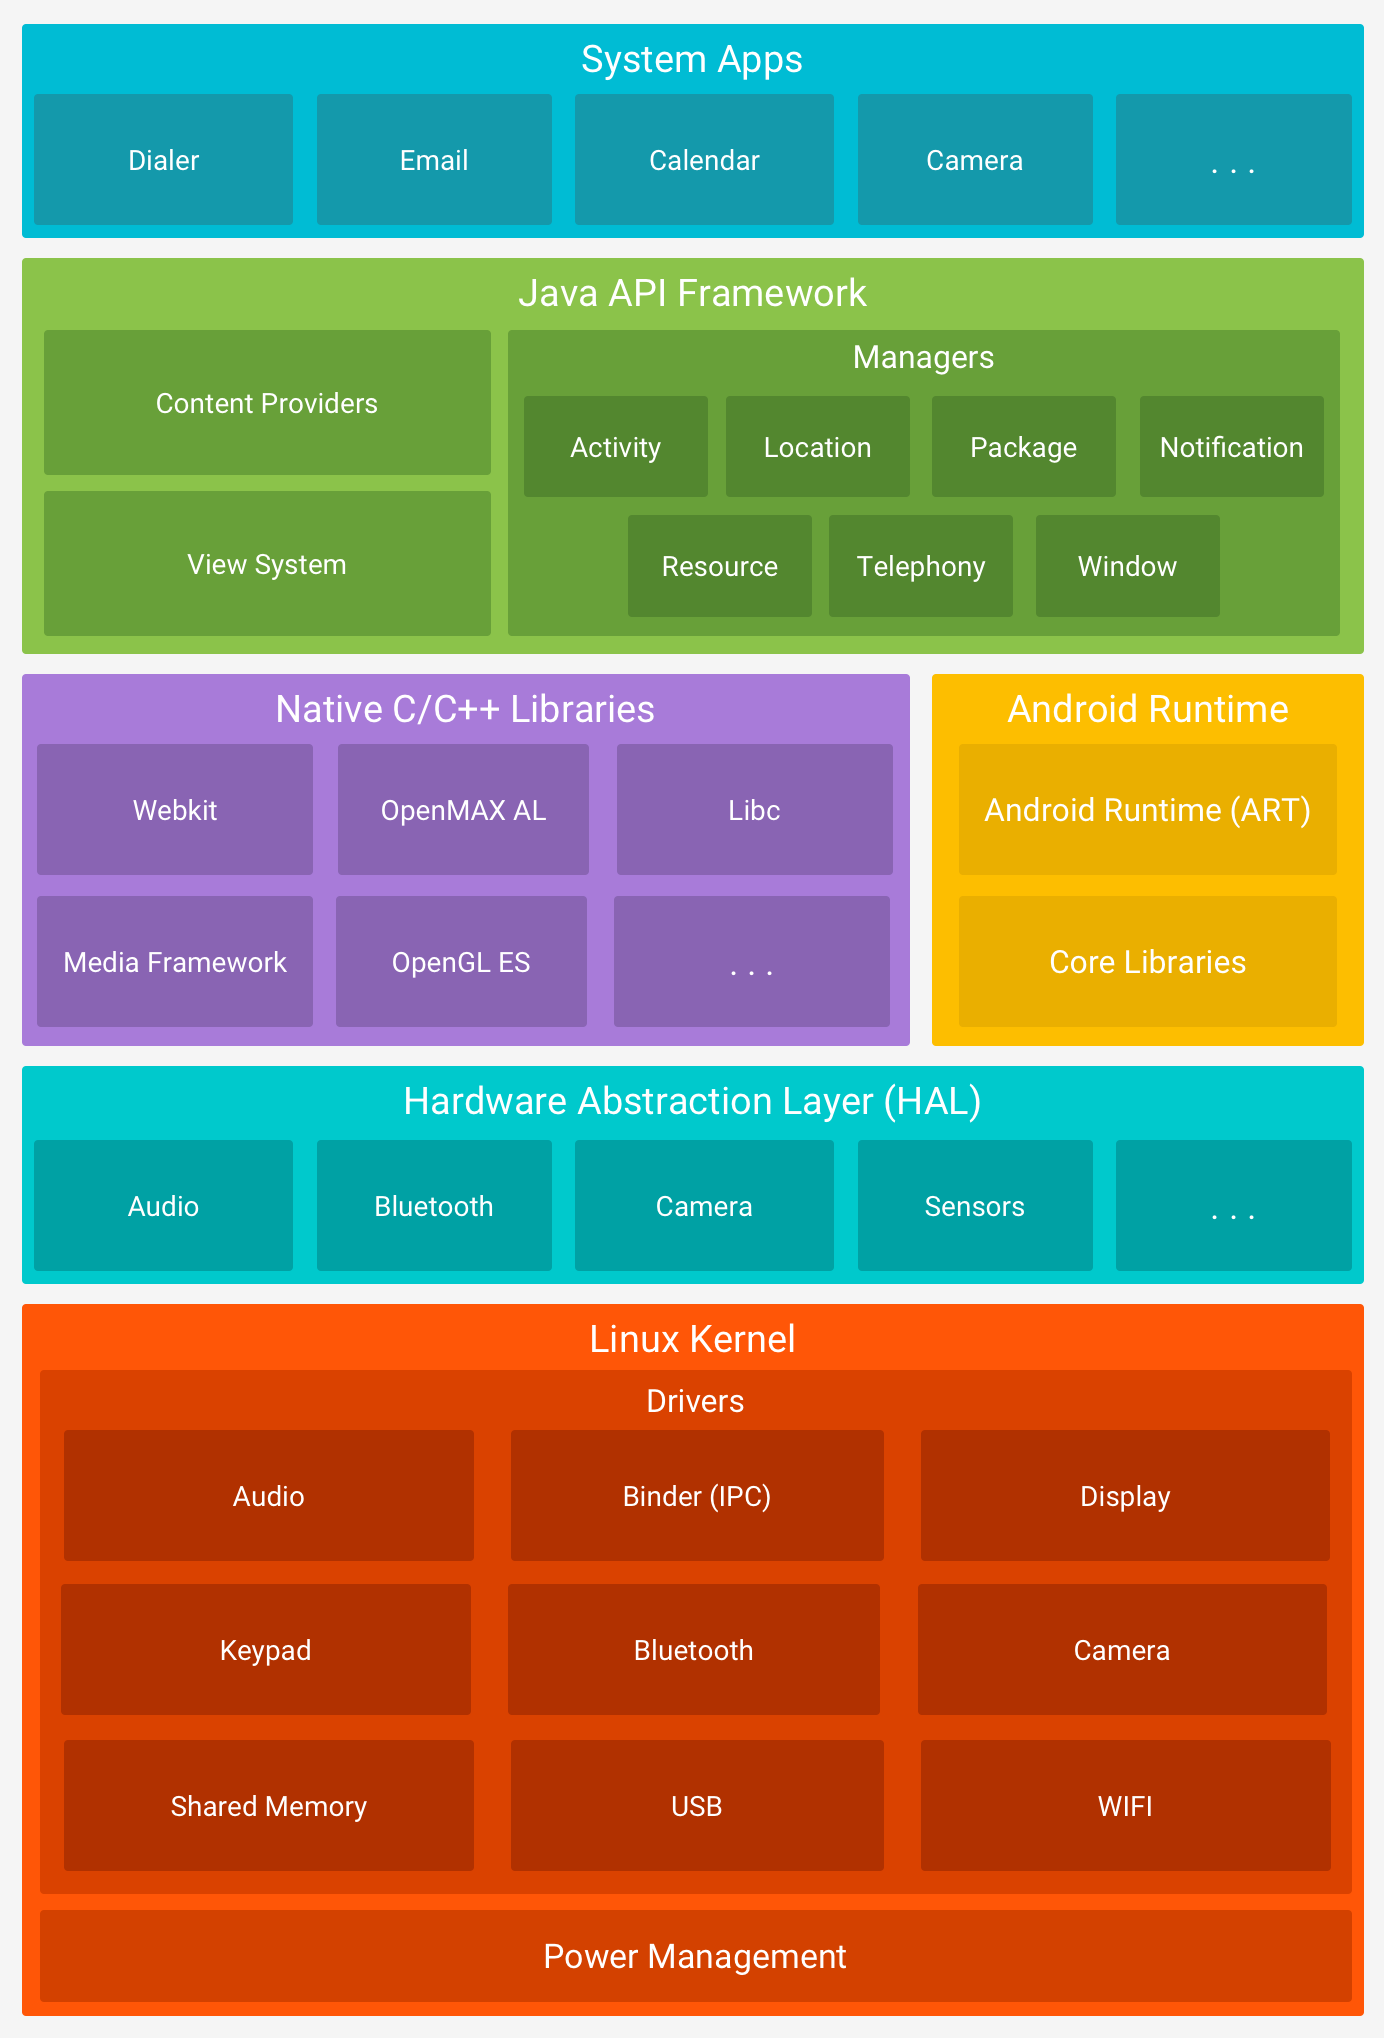
\includegraphics[width=1.0\textwidth]{android_platform_arch.png}  
    \caption{Компоненты платформы Android}
	\label{fig:android_platform_arch}
\end{figure}

\subsection{История версий Android}
\label{sub:android_platform:history}

История развития ОС Android насчитывает около 15 лет.
Первая стабильная версия данной операционной системы (Android 1.0) вышла в сентябре 2008 года \cite{android_first_release}.
Начиная с версии Android 1.5 <<Cupcake>>, среди разработчиков появилась традиция присваивать значительным выпускам системы названия, связанные со сладостями: Android 1.6 <<Donut>> (англ. \textit{пончик}), Android 4.4 <<KitKat>>, Android 8.0 <<Oreo>> и т. д.
Однако с версии Android 10 от этой традиции отказались \cite{android_codenames}.

За годы развития ОС Android постепенно приобретала много новых функций и возможностей.
Каждое улучшение по отдельности может показаться не очень значительным, однако в комплексе они значительно улучшают пользовательский опыт (UX) и упрощают взаимодействие с устройством.


\subsubsection{}
\label{subsub:android_platform:history:kitkat}

\textit{Android 4.4 <<KitKat>>} вышла в декабре 2013 г. \cite{android_release_notes} и по количеству новых возможностей была одной из самых революционных версий Android в то время.
Среди добавленных возможностей и улучшений:
\begin{itemize}
	\item Host Card Emulation для NFC (эмуляция платёжных карт);
	\item печать документов и изображений по Wi-Fi или с помощью облачных сервисов (например, Google Cloud Print);
	\item Storage Access Framework -- контролируемый доступ к пользовательским файлам из сторонних приложений;
	\item новое API для управления SMS;
	\item использование Chromium в качестве движка для Android WebView (быстрее устаревшей реализации на основе WebKit);
	\item запись видео с экрана и др. \cite{android_kitkat}
\end{itemize}


\subsubsection{}
\label{subsub:android_platform:history:lollipop}

\textit{Android 5.0 <<Lollipop>>} была выпущена в октябре 2014 г. \cite{android_release_notes}
Наиболее значительные улучшения в этой версии:
\begin{itemize}
	\item стандартизированный пользовательский интерфейс, построенный на принципах Material Design;
	\item некоторые оповещения теперь могут отображаться на экране блокировки (например, оповещения о пропущенных вызовах, сообщениях и т. п.);
	\item экран просмотра запущенных приложений сделан более удобным и понятным для пользователей;
	\item поддержка графического API OpenGL ES 3.1;
	\item работа со звуком с малой задержкой (англ. \textit{low latency audio});
	\item просмотр и запись видео с использованием кодека H265 и др. \cite{android_lollipop}
\end{itemize}


\subsubsection{}
\label{subsub:android_platform:history:oreo}

\textit{Android 8.0 <<Oreo>>} была представлена общественности в августе 2017 г. \cite{android_release_notes}
Основные возможности, реализованные в 8.0:
\begin{itemize}
	\item режим <<картинка в картинке>> (в основном используется для показа видео в фоновом режиме при совершении других действий с устройством);
	\item значительные улучшения системы оповещений (возможность заблокировать показ оповещений от определённого приложения и др.);
	\item использование дополнительных шрифтов, установленных вместе со сторонним приложением;
	\item возможность более тонкой настройки разрешений, предоставленных каждому из приложений и др. \cite{android_oreo}
\end{itemize}


\subsubsection{}
\label{subsub:android_platform:history:pie}

\textit{Android 9 <<Pie>>} вышла в августе 2018 г. \cite{android_release_notes}
Список новых функций, добавленных в версии Android 9 <<Pie>>:
\begin{itemize}
	\item навигация внутри зданий с помощью Wi-Fi RTT;
	\item поддержка экранов с вырезом для динамика в верхней части;
	\item одновременный доступ к видеопотоку с нескольких камер;
	\item переработан API, связанный с декодированием изображений (добавлен класс ImageDecoder, а BitmapFactory объявлен устаревшим);
	\item сжатие изображений с использованием алгоритма HEIF/HEIC;
	\item API для работы с искусственными нейронными сетями и др. \cite{android_pie}
\end{itemize}


\subsubsection{}
\label{subsub:android_platform:history:android_10}

\textit{Android 10} -- последняя стабильная версия Android.
Она вышла совсем недавно, в июле 2020 г. \cite{android_release_notes}
Главные нововведения в этой версии:
\begin{itemize}
	\item поддержка устройств со складным экраном;
	\item поддержка сетей 5G;
	\item быстрые ответы на сообщения на основе машинного обучения;
	\item общесистемная тёмная тема;
	\item расширенное управление с помощью жестов;
	\item более тонкий контроль над данными о местоположении, собираемыми сторонними приложениями;
	\item шифрование пользовательских данных по умолчанию;
	\item обязательная поддержка графического API Vulkan 1.1 и др. \cite{android_10}
\end{itemize}


\subsubsection{}
\label{subsub:android_platform:history:android_11}

\textit{Android 11} -- версия Android, которая на данный момент (декабрь 2020 г.) пока находится в разработке.
Среди заявленных возможностей:
\begin{itemize}
	\item новое API ImageDecoder для Android NDK;
	\item API для доступа к текущей частоте кадров;
	\item улучшенная поддержка закруглённых экранов и др. \cite{android_11}
\end{itemize}

\subsubsection*{}
\label{subsub:android_platform:history:distribution}

К сожалению, производители мобильных устройств на базе ОС Android выпускают обновления ОС для своих продуктов в течение ограниченного периода времени.
По прошествии этого периода установить более новую версию Android либо очень сложно (требуются специальные знания), либо вовсе невозможно.
Поэтому в мире значительный процент устройств работает на устаревших версиях Android.
К счастью, в последнее время ситуация с обновлениями ОС стала улучшаться, и процент устройств с устаревшими версиями неуклонно снижается.
На рисунке~\ref{fig:android_distribution_dashboard} представлена статистика по используемым версиям Android. \cite{android_about_dashboards}

\begin{figure}[ht]
    \centering
    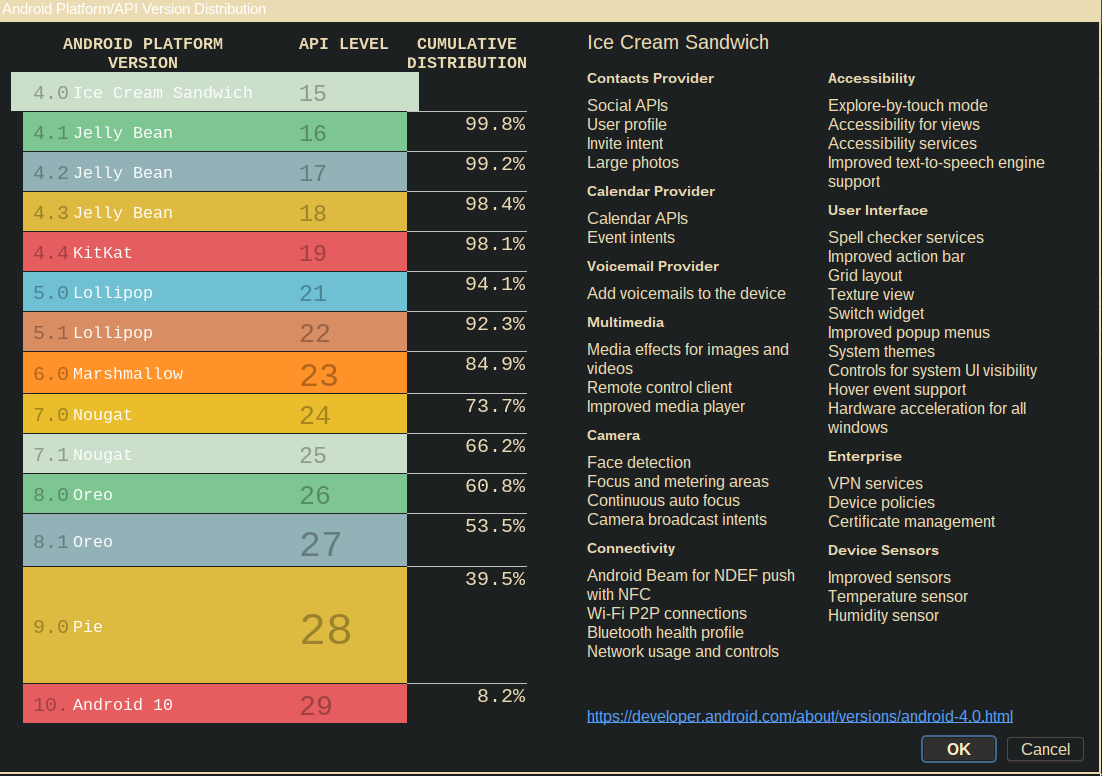
\includegraphics[width=1.0\textwidth]{android_distribution_dashboard.png}
	\caption{Распределение версий Android}
	\label{fig:android_distribution_dashboard}
\end{figure}

Из данного изображения следует, что 98,1\% Android-устройств используют версию 4.4 и выше.
На последней стабильной версии (Android 10) пока работает всего 8,2\% от всех устройств.

\subsection{Сравнение Android с другими мобильными платформами} \label{sub:android_platform:comparison}

ОС Android существует уже более 15 лет, но её популярность стала расти особенно быстрыми темпами с 2011 года, когда рыночная доля Android превысила отметку 50\% и достигла 52,9\%.
К концу 2012 года Android заняла 70\% рынка мобильных ОС, главным образом за счёт сокращения доли ОС Symbian от Nokia и BlackBerry.
С тех пор доля Android остаётся вблизи данной отметки.
В таблице \ref{table:android_platform:comparison:market_share} представлена доля рынка мобильных ОС в 2011 -- 2012 годах. \cite{comparative_study_of_mobile_oses_2016}

\begin{table}[ht]
	\caption{Рыночная доля мобильных ОС в 2011 -- 2012 годах}
	\label{table:android_platform:comparison:market_share}
	\centering
	\begin{tabular}{| l | l | l |}
		\hline
		\thead{ОС} & \thead{Доля в \\ конце 2011 г., \%} & \thead{Доля в \\ конце 2012 г., \%}\\
		\hline Android		 & 52,9 & 70,1 \\                                             
		\hline iOS		     & 23,0 & 21,1 \\
		\hline BlackBerry	 & 8,1\ & 3,2 \\
		\hline Windows Phone & 1,5\ & 2,6 \\
		\hline Другие		 & 14,5 & 3,0 \\
		\hline
	\end{tabular}
\end{table}

На сегодняшний день фактически единственным конкурентом Android на рынке мобильных операционных систем является iOS с долей 28\% от компании Apple.
К сожалению, доля других ОС находится на уровне статистической погрешности \cite{statcounter_mobile_os}.
Сформировавшаяся дуополия Android и iOS, безусловно, отрицательно сказывается на качестве данных ОС, поскольку при отсутствии достаточно популярных конкурентов у Android и iOS нет стимула для того, чтобы внедрять какие-либо по-настоящему революционные возможности, вместо заимствования идей друг у друга.

У такой большой популярности Android есть ряд причин, среди них:
\begin{itemize}
	\item эффективный механизм автоматического управления памятью (система автоматически переводит неактивные приложения в режим сна для сохранения заряда батареи);
	\item безопасность и изоляция приложений друг от друга с использованием механизмов, предоставляемых ядром Linux (создание отдельного пользователя для каждого приложения, SELinux, система разрешений и др.);
	\item спонсирование разработки Android корпорацией Google, одной из крупнейших технологических компаний в мире;
	\item открытый исходный код и широкие возможности для настройки системы под себя опытными пользователями (в отличие от Apple iOS, в которой права пользователя максимально ограничены).
\end{itemize}

Как правило, поддержка крупной компании является немаловажным фактором для успеха программного продукта.
Поэтому альтернативы Android на базе Linux, развиваемые сообществом -- postmarketOS, UBPorts (ранее Ubuntu Touch) -- пока, к сожалению, не готовы для повседневного использования, главным образом из-за проблем с закрытыми драйверами оборудования.
Пока невозможно совершать звонки, пользоваться камерой, GPS и др. функциями на большинстве моделей смартфонов.

Относительно недавно компанией Purism был представлен смартфон \textit{Librem 5}.
Librem 5 максимально использует свободное ПО, поставляется с предустановленным дистрибутивом Linux PureOS (см. рисунок \ref{fig:librem5}).
Заявлена возможность подключения к Librem 5 внешнего монитора, клавиатуры и мыши с последующим использованием в качестве полноценного компьютера.
Интерфейс приложений специально разрабатывается с оглядкой на адаптивность к разным размерам экрана.
Кроме того, Librem 5 оснащён аппаратными выключателями радиомодулей для ситуаций, когда пользователь хочет минимизировать риск отслеживания через смартфон.

\begin{figure}[ht]
    \centering
    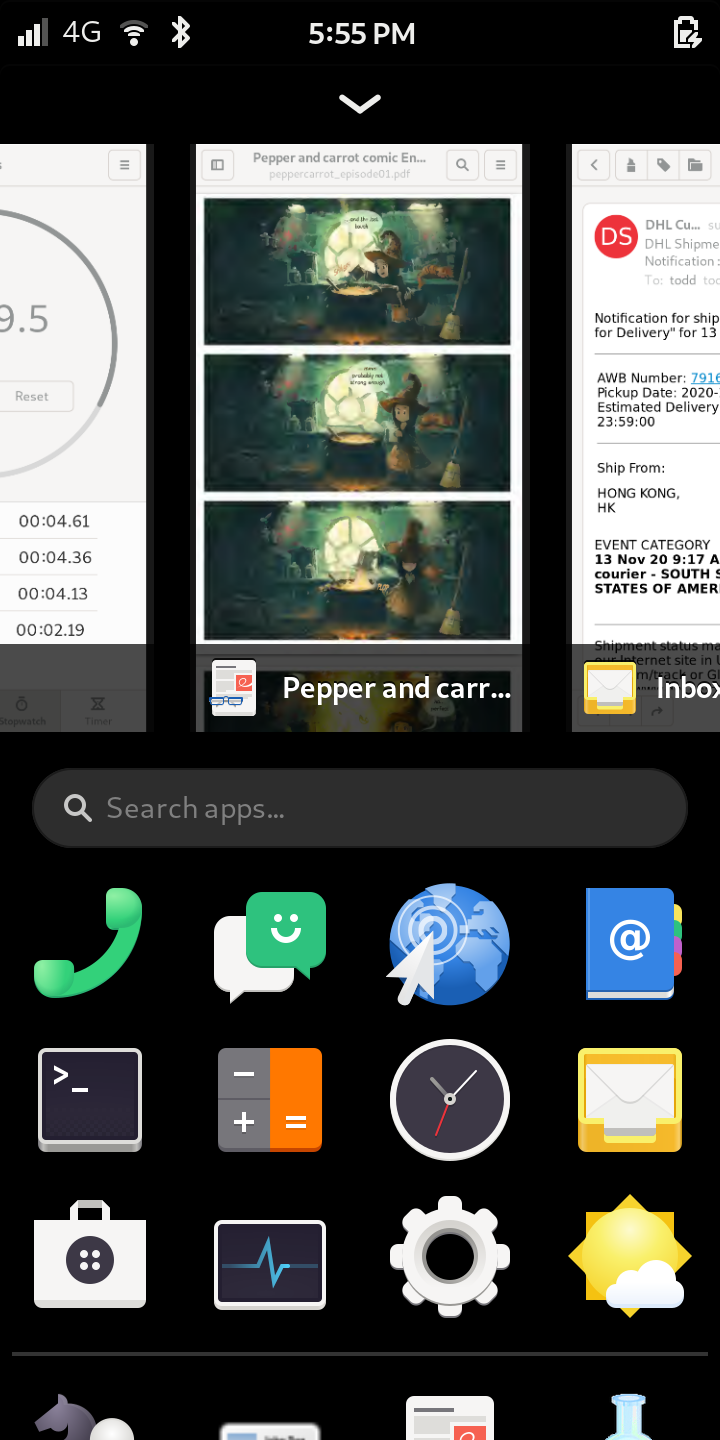
\includegraphics[width=0.3\textwidth]{librem5.png}  
    \caption{Внешний вид интерфейса Librem 5 с PureOS}
	\label{fig:librem5}
\end{figure}

Среди минусов Librem 5 -- довольно высокая цена в \$799 \cite{librem5}.
Такая цена главным образом обусловлена малым объёмом первой выпущенной партии, а также тем, что Purism самостоятельно разрабатывает не только программное, но и аппаратное обеспечение для устройства.
